\documentclass[standalone, version=2.0]{huangfusl-template}
\begin{document}
\begin{tabular}{ccc}
    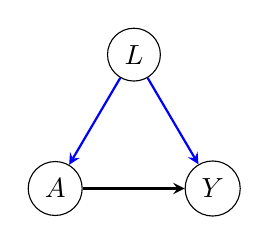
\begin{tikzpicture}
        \node[circle, draw] (L) at (0, 0) {$L$};
        \node[circle, draw] (A) at (-1, -1.7) {$A$};
        \node[circle, draw] (Y) at (1, -1.7) {$Y$};

        \draw[-stealth, thick, draw=blue] (L) -- (A);
        \draw[-stealth, thick, draw=blue] (L) -- (Y);
        \draw[-stealth, thick] (A) -- (Y);
    \end{tikzpicture} &
    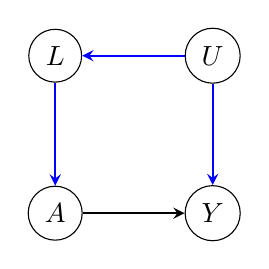
\begin{tikzpicture}
        \node[circle, draw] (L) at (-1, 1) {$L$};
        \node[circle, draw] (U) at (1, 1) {$U$};
        \node[circle, draw] (A) at (-1, -1) {$A$};
        \node[circle, draw] (Y) at (1, -1) {$Y$};

        \draw[-stealth, thick, draw=blue] (L) -- (A);
        \draw[-stealth, thick, draw=blue] (U) -- (Y);
        \draw[-stealth, thick] (A) -- (Y);
        \draw[-stealth, thick, draw=blue] (U) -- (L);
    \end{tikzpicture} &
    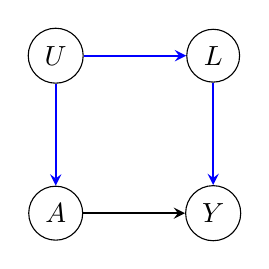
\begin{tikzpicture}
        \node[circle, draw] (L) at (1, 1) {$L$};
        \node[circle, draw] (U) at (-1, 1) {$U$};
        \node[circle, draw] (A) at (-1, -1) {$A$};
        \node[circle, draw] (Y) at (1, -1) {$Y$};

        \draw[-stealth, thick, draw=blue] (L) -- (Y);
        \draw[-stealth, thick, draw=blue] (U) -- (A);
        \draw[-stealth, thick] (A) -- (Y);
        \draw[-stealth, thick, draw=blue] (U) -- (L);
    \end{tikzpicture}
    \end{tabular}
\end{document}